% Asset ID: A22ProjectilesTikZ-006
% Purpose: Show two projectile paths meeting at the same point and time.
\documentclass[tikz,border=8pt]{standalone}
\usepackage{amsmath}
\usetikzlibrary{arrows.meta,calc}
\begin{document}
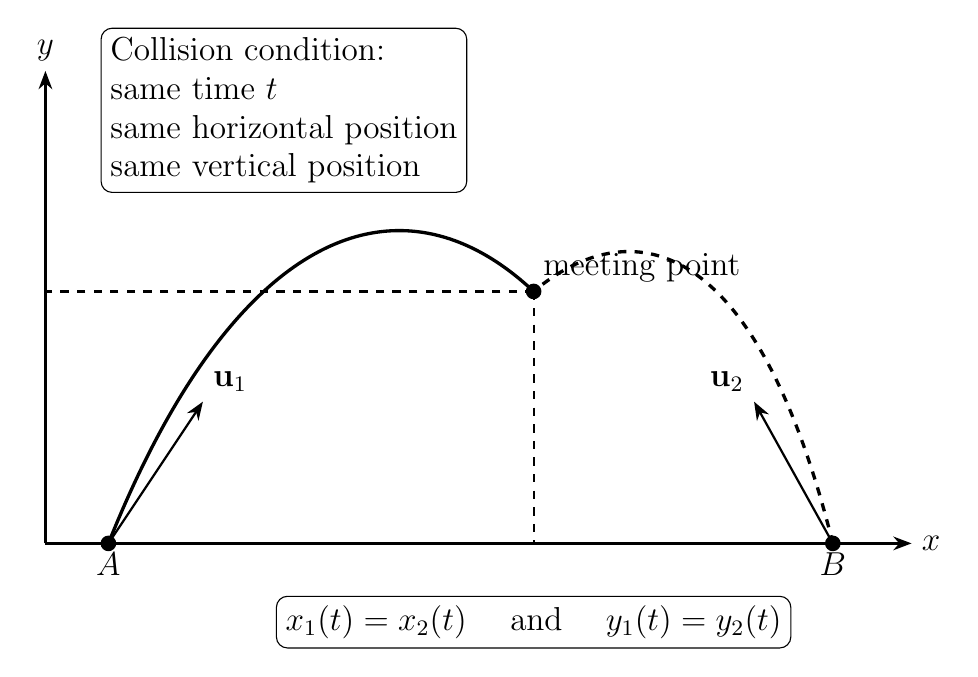
\begin{tikzpicture}[>=Stealth,axis/.style={->,thick},pathA/.style={very thick},pathB/.style={very thick,dashed},arrow/.style={->,thick},guide/.style={dashed,thick},label/.style={font=\large},point/.style={circle,fill=black,inner sep=2pt}]
\draw[axis] (0,0)--(11,0) node[right,label] {$x$}; \draw[axis] (0,0)--(0,6) node[above,label] {$y$};
\coordinate (A) at (0.8,0); \coordinate (B) at (10.0,0); \coordinate (M) at (6.2,3.2);
\node[point] at (A) {}; \node[point] at (B) {}; \node[point] at (M) {};
\node[below,label] at (A) {$A$}; \node[below,label] at (B) {$B$}; \node[above right,label] at (M) {meeting point};
\draw[pathA] (A) .. controls (2.4,4.0) and (4.5,4.8) .. (M); \draw[pathB] (B) .. controls (9.0,4.0) and (7.4,4.2) .. (M);
\draw[arrow] (A)--++(1.2,1.8) node[above right,label] {$\mathbf{u}_1$}; \draw[arrow] (B)--++(-1.0,1.8) node[above left,label] {$\mathbf{u}_2$};
\draw[guide] (M)--(6.2,0); \draw[guide] (M)--(0,3.2);
\node[draw,rounded corners,align=left,font=\large,anchor=west] at (0.7,5.5) {Collision condition:\\same time $t$\\same horizontal position\\same vertical position};
\node[draw,rounded corners,align=center,font=\large,minimum width=6.5cm] at (6.2,-1.0) {$x_1(t)=x_2(t)$ \quad and \quad $y_1(t)=y_2(t)$};
\end{tikzpicture}
\end{document}
